\begin{figure}[t]
    \centering
    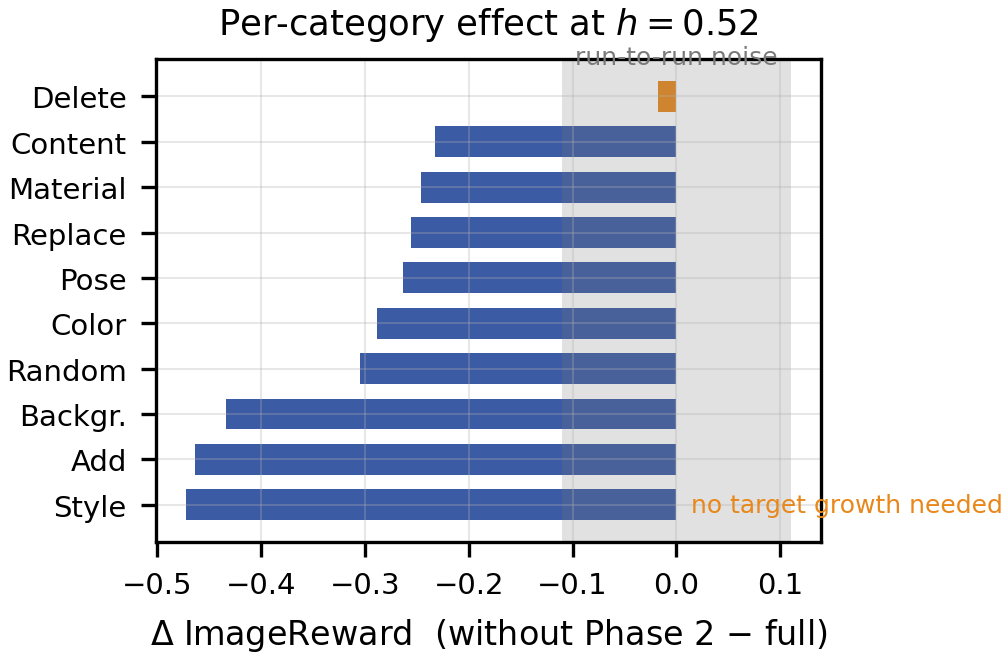
\includegraphics[width=\linewidth]{imgs/fig_beta_category.png}
    \caption{Per-category effect of removing Phase~2 at $h{=}0.52$. The shaded band is the run-to-run noise scale for a category of this size. \texttt{Delete} is the one category whose target needs no region absent from the source, and it is the one category inside the noise band --- an internal control showing the other losses are not an artifact of the ablated code path. The three largest losses are exactly the categories whose target content must grow outside the source focus region.}
    \label{fig:beta_category}
\end{figure}
